\chapter{Exploring Light and Lenses}
\thispagestyle{fancy}
\fancyhead[RE,LO]{Experiment \thechapter}
%
Optics — the sub-field of physics focusing on the study of light — is important to many areas of biology, including vision, ecology, botany, neurobiology and molecular biology. 
The use of optics in biology has evolved from the simple light microscope used by Darwin to the complex, live-cell, high resolution microscopes used in current cutting-edge research. 
In this two-week lab, we will be exploring the behavior of light and lenses. 
Microscopes usually employ at least two lenses together—but, as we are only beginning to learn about light, we will be exploring single-lens systems. 
\par 
%Your task is two-fold: 1) Design a way of determining the focal lengths, f, for five converging (bi-convex) lenses; and then, 2) Design an experiment to explore how the focal length, f, of a lens interacts with the image distance, i, and object distance, o, when the total distance, from object to image, is a fixed length, L. 
\begin{figure}[hbtp]
\centering
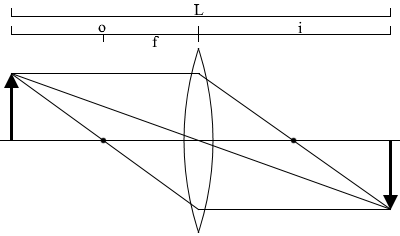
\includegraphics[width=0.5\textwidth]{lensDiagram}
\caption{Ray diagram of a single-lens system.}
\label{fig:lensDiagram}
\end{figure}

A typical single-lens system is shown in figure~\ref{fig:lensDiagram}. The image distance, $i$, is the distance from the location of the image to the center of the lens. 
The object distance, $o$, is the distance from the location of the object to the center of the lens. 
For most microscopes, the object location and image location cannot be changed (they are a fixed distance, $L$ apart), so it is the type of lens (and thus its focal length, $f$) and the location of the lens that are changed to achieve different magnifications and to focus the image. 
Ultimately, you should be able to construct a mathematical model of the interaction of focal length and image/object distance that is supported by your data. 
Think carefully about your experimental designs and how they affect your sources (and values!) of uncertainty.

\paragraph{For this two week lab:} Your overall task for the next two weeks is to design a way of determining the focal lengths for five converging (bi-convex) lenses.
Then, design an experiment to explore how the focal length of a lens interacts with the image distance and object distance when the total distance from object to image is a fixed length.
You will do this in multiple stages:
\begin{enumerate}
\itemsep-0.2em
\item Get familiar with the optical equipment. Make sure that the lenses are clean, if they are not, ask your TA for help cleaning them.
\item Determine the focal lengths of your lenses.
\item Explore how the focal length of a lens interacts with the image distance and object distance when the total length from object to image is fixed.
\end{enumerate}

\section*{About the Equipment:}
Each group has access to:
\begin{itemize}
\itemsep-0.3em
\item a light source (your object) with pole clamp,
\item five converging (bi-convex) lenses of differing focal lengths,
\item one diverging (bi-concave) lens,
\item a lens holder with pole clamp,
\item a long optical rail (pole) with table clamp,
\item small LED light boxes emitting different colors of light,
\item a light box with a plano-convex lens,
\item a meter stick and a ruler, and
\item a simple light microscope à la Darwin.
\end{itemize}
Be sure that your optical elements, such as lenses, are carefully aligned with the vertical axis of your equipment. 
If you need help with this, or are not sure why this is important, please ask a TA/LA. 
Additionally, please be gentle with the equipment, especially the glass lenses, and try to avoid getting finger-prints, skin oils, or dirt on the lenses. Do not over-tighten clamps — if you are unsure, ask for help.
\paragraph*{Things to consider including in your lab report:} In your lab write-up, you may want to include careful discussions of:
\begin{itemize}
\itemsep-0.3em
\item your methods for finding the focal lengths and investigating the $f/i/o$ relationships
\item your data and your analysis of the data
\item your mathematical model for the interaction of focal length and image/object distances
\item your comparison of your work with the work of other groups, as well as your critique of your experiment and conclusions. 
\end{itemize}
You may also want to include hand-drawn elements (such as ray diagrams).